%implementing document formatting:
\input{settings/preamble.tex}
\begin{document}

%including front page:
\clearpage
\thispagestyle{empty}

\begin{figure}[H]
	\raggedleft
		\includegraphics[width=0.2\textwidth]{figures/aaulogo-en.png}
\end{figure}
\vspace*{\fill} 
\begin{center}
\begin{Huge}
P5 Project Report - Autumn 2015\\
\vspace{5 mm}
\textbf{??\fxnote{Input project title}}\\
\vspace{3 mm}
Group ??\fxnote{Input group number}
\end{Huge}
\end{center}
\vspace*{\fill}

\begin{center}
\line(1,0){400}
\end{center}
%clears one or two pages to make the document start on right hand side:
\cleardoublepage

%numbers the pages with Roman numeral - starts from "i":
\frontmatter

%including title sheet:
%\begin{document} 
\thispagestyle{empty}
%\begin{titlepage}
\begin{nopagebreak}
{\samepage 

\begin{tabular}{r}
\parbox{\textwidth}{  \raisebox{11mm}{\includegraphics[height=1.5cm]{figures/aaulogo-en.png}}
\hfill \hspace{2cm} \parbox{8cm}{\begin{tabular}{l} %4.90
{\small \textbf{\textcolor{MidnightBlue}{\colorbox{white}{5\textsuperscript{th} Semester}}}}\\
{\small \textbf{\textcolor{MidnightBlue}{School of Information and}}}\\
{\small \textbf{\textcolor{MidnightBlue}{Communication Technologies}}}\\ 
{\small \textbf{\textcolor{MidnightBlue}{Electronics and IT}}}\\
{\small \textcolor{NavyBlue}{Fredrik Bajers Vej 7B}} \\
{\small \textcolor{NavyBlue}{9220 Aalborg}} \\
{\small \textcolor{NavyBlue}{\emph{http://www.sict.aau.dk/electronics-and-it}}}
\end{tabular}}}
\end{tabular}

\begin{tabular}{cc}
\parbox{7cm}{
\begin{description}

\item {Title:}

??\fxnote{Input project title}\\

\item {Theme:} 

\small{
Digital and Analog Systems\\
Interacting with the Surroundings
}

\end{description}

\parbox{8cm}{

\begin{description}
\item {Project Period:}\\
   P5, Autumn 2015\\
   02/09/2015 - 17/12/2015\\
   
\item {Project Group:}\\
  ??\fxnote{Input group number}\\
  
\item {Participants:}\\
Amalie V. Petersen\\
Julien Brehin\\
Mads Gotthardsen\\
Niels Skov Vestergaard\\
Romaric Destremau\\
Thomas Rasmussen\\
\hspace{2cm}
\item {Supervisor:}\\
??\fxnote{Input supervisor}
\end{description}
}
\begin{description}
\item {Prints: ??}\fxnote{Input number of prints}
\item {Pages: ??}\fxnote{Input number of pages}
\item {Appendices: ??}\fxnote{Input number of appendices}
\item {Concluded 17/12/2015}
\end{description}
\vfill } &
\parbox{7cm}{
  \vspace{.15cm}
  \hfill 
  \begin{tabular}{l}
  {Synopsis}\bigskip \\
  \fbox{
    \parbox{6.5cm}{\bigskip
     {\vfill{\small In order to facilitate the lawn mowing, robotic lawn mowers have been pushed to the market the last few years.\\
From a given vehicle base, this project intends to improve the easiness of use and reduce installation constraints by use of ultrasound positioning and wireless communication.\\
Models of this vehicle have been built, upstream from the design and implementation of appropriate controllers to actually make the vehicle autonomous. The prototype is implemented with a positioning system which communicates with an Arduino platform running an open-source kernel. Feedback is fed to the controllers from angular and velocity sensors for which filtering has been considered.\\
Except from one functionality which could not be tested in practice due to one sensor incompatibility with indoor environment. The different parts of the system have been simulated through software and have been proven to work successfully in real life.
     \bigskip}}
     }}
   \end{tabular}}
\end{tabular}} \vspace{1.3cm}
\raggedleft
\textit{\tiny Publication of this report's contents (including citation) without permission from the authors is prohibited.}\nopagebreak
\\
\end{nopagebreak}
%\end{titlepage}
%\end{document}

\cleardoublepage

\chapter*{Preface}
The project is to design a autonomous vehicle able to 

Text by:\\
%
\begin{table}[H]
	\centering
		\begin{tabular}{c c c}
			\underline{\phantom{JAERJAERJAERJAERGO}} & \phantom{cookies} & \underline{\phantom{JAERJAERJAERJAERGO}} \\
			Amalie V. Petersen			& \phantom{cookies} & Julien Br\'ehin		\\
			&&\\
			&&\\
			\underline{\phantom{JAERJAERJAERJAERGO}} & \phantom{cookies} & \underline{\phantom{JAERJAERJAERJAERGO}} \\
			Mads Gotthardsen			& \phantom{cookies} & Niels Skov Vestergaard		\\
			&&\\
			&&\\
	    \underline{\phantom{JAERJAERJAERJAERGO}} & \phantom{cookies} & \underline{\phantom{JAERJAERJAERJAERGO}} \\
			Romaric Destremau 					& \phantom{cookies} & Thomas Rasmussen 			\\			
		\end{tabular}
\end{table}

\cleardoublepage

%the '*' allows the tableofcontents to be excepted from being indexed in table of contents.
\tableofcontents*

%numbers the pages with Arabic numeral - starts from 1.
\mainmatter

%---------- Part 1 ----------------------------------------
\part{Introduction}
\chapter{Introduction}
\section{Household robots in general}
More and more robots appear in everyday life. Automatic vacuum cleaners and floor washers are getting widespread, as the technology is becoming cheaper and better. The vacuum cleaners have matured to a level, where they are been considered for saving man-hours in the elderly care sector.\\

\noindent
Outside the walls of our homes lays the next weekly hurdle: Mowing the lawn. A known way to handle this, is to pay the neighbour's teenager to do it. Unfortunately they grow up and move out, leaving the lawns in the residential neighbourhoods behind.\\ 

\noindent
Luckily engineers has stepped in, and provided a more long-term solution: Robotic lawn mowers.

\section{Robotic lawn mowers}
Several manufacturers of electrical gardening machines have started selling robotic lawn mowers in the recent years. In general they use one of two strategies when cutting the lawn:
\begin{itemize}
	\item Random direction mowers
	\item Parallel line mowers
\end{itemize}

\noindent
Mowers using the random direction strategy will drive in a straight line until a guard wire or an obstacle is detected. They will then turn in a random direction, and continue. See \figref{fig:randomcut}

\begin{figure}[H]
\centering
\includegraphics[scale=0.8]{figures/noLogicut.jpg} 
\label{fig:randomcut}
\caption{Random cut system [source:Bosch]} 
\end{figure}

\noindent
When the battery is nearly discharged, the mower will follow the guard wire back to the base station for recharging.\\

\noindent
Parallel line mowers uses a more intelligent control algorithm to optimize the mowing. After an initial learning run, following the guard wire around the lawn to be mowed, it will map the lawn, and cut in parallel lines, see \figref{fig:logicut}. The advantage of this strategy efficiency, as the lawn mower will not run over the same spots more than once. According to Bosch, a given lawn can be mowed up to 30\% faster with their Logicut system.
%% TODO: Insert source
 

\begin{figure}[H]
\centering
\includegraphics[scale=0.8]{figures/logicut.jpg} 
\label{fig:logicut}
\caption{Bosch Logicut system [source:Bosch]} 
\end{figure}

\noindent
Common for both systems is the guard wire, which has to be placed around the lawn and anywhere the lawn mower is not allowed to go, like flower beds, swimming pools, etc. \\

\noindent
This brings us to the problem with existing products.

\section{Problems with existing robotic lawn mowers}
All commercially available robotic lawn mowers requires a guard wire placed around the lawn. This can either be placed at the surface, and be held in place by pegs, or dug down below the surface. The guard wire must be routed around flower beds, etc. as well, see \figref{fig:robomow}

 
\begin{figure}[H]
\centering
\includegraphics[scale=0.6]{figures/robomow.png} 
\label{fig:robomow}
\caption{Guard wire installation [source:Robomow]} 
\end{figure}
\noindent

The use of the guard wire for guiding the mower back to the charging station presents another potential problem: In a garden with many restricted areas, the guard wire could get very long. This could therefore make the journey home long, compared to a more direct route. This again uses more battery power, that instead could have been used for actually mowing the lawn.\\

\noindent
This will be the motivation for the project: To avoid the work routing a wire around the garden, and as a bonus get more work done on a battery charge, by not wasting power following the wire home. 
    
\section{The Games on Track (GoT) system}
We were provided with the 'Games on Track GT-Position' system as a start to be able to figure out the lawn mower position in space.\\\\
It is composed of four different parts both hardware and software :
\begin{itemize}
	\item The tracked module, which emits ultra-sound waves. It should be placed on our lawn mower itself, so that the emitting cell is not obstructed by anything.
	\item Some beacons or receivers, placed all around the place the lawn mower will move in. Depending on the terrain, we can use from 2 to more than 20 of these : the more we place, the more accuracy we can get to fight against any ambient noise.
	\item The central system which gathers information about the distance of the tracked module to each beacon and transmits it to the computer via USB in regular intervals.
	\item The GoT software aggregates the received positions thoughout time and can be used to draw a map of the terrain (the lawn) and send every needed information to a third-party (our) piece of software.
\end{itemize}
GoT was firstly designed for train modeling but it is easily adaptable for any use of position tracking and seems a good choice, at first, for our autonomous lawn mower.

\section{Why not satellite positioning system ?}
The reasons why satellite positioning system won't be used in our project are mainly related to accuracy and energy consumption.\\\\
Indeed, these kinds of system like GPS or GLONASS would require a dedicated chip to put on the final system. The problem then would be the lack of precision under a few meters (around 2 or 3 meters in ideal situations for the best chips). \\\\
% TODO : Add reference to "A Review of GLONASS" Miller, 2000 & http://www.gps.gov/systems/gps/performance/accuracy/ %
Moreover, this kind of system implies slow communications with different distant satellites at the same time. Therefore, the energy consumption would quickly rise, thus reducing the lawn mower autonomy, which is not desirable.

\section{Potential consumer expectations}
The design of a product has no real value if no one is interested in using it. Thus, choices made during this project have to be made in accordance with the final user's expectations.\\\\
For instance, we need to keep in mind considerations regarding the autonomy of the vehicle (both in energy and for the navigation), but also towards the overall cost (\emph{insert price approximation here}). Even though, the GoT system itself has a cost beyond anything a normal customer would pay for a lawn mower, it appears, at first, as a good solution for us in terms of accuracy and energy consumption compared to GPS-like systems which are also quite expensive (\emph{insert price approximation here}). \\\\
For an improvement, we could consider replacing it with a similar solution as it is only a simple brick of the whole system. \emph{(This sentence should be perhaps moved to a dedicated part of the report)}\\\\
These are the types of preliminary considerations that will influence our design process for an autonomous lawn mower.

%---------- Part 2 ----------------------------------------
%\chapter{Introduction}
\section{Household robots in general}
More and more robots appear in everyday life. Automatic vacuum cleaners and floor washers are getting widespread, as the technology is becoming cheaper and better. The vacuum cleaners have matured to a level, where they are been considered for saving man-hours in the elderly care sector.\\

\noindent
Outside the walls of our homes lays the next weekly hurdle: Mowing the lawn. A known way to handle this, is to pay the neighbour's teenager to do it. Unfortunately they grow up and move out, leaving the lawns in the residential neighbourhoods behind.\\ 

\noindent
Luckily engineers has stepped in, and provided a more long-term solution: Robotic lawn mowers.

\section{Robotic lawn mowers}
Several manufacturers of electrical gardening machines have started selling robotic lawn mowers in the recent years. In general they use one of two strategies when cutting the lawn:
\begin{itemize}
	\item Random direction mowers
	\item Parallel line mowers
\end{itemize}

\noindent
Mowers using the random direction strategy will drive in a straight line until a guard wire or an obstacle is detected. They will then turn in a random direction, and continue. See \figref{fig:randomcut}

\begin{figure}[H]
\centering
\includegraphics[scale=0.8]{figures/noLogicut.jpg} 
\label{fig:randomcut}
\caption{Random cut system [source:Bosch]} 
\end{figure}

\noindent
When the battery is nearly discharged, the mower will follow the guard wire back to the base station for recharging.\\

\noindent
Parallel line mowers uses a more intelligent control algorithm to optimize the mowing. After an initial learning run, following the guard wire around the lawn to be mowed, it will map the lawn, and cut in parallel lines, see \figref{fig:logicut}. The advantage of this strategy efficiency, as the lawn mower will not run over the same spots more than once. According to Bosch, a given lawn can be mowed up to 30\% faster with their Logicut system.
%% TODO: Insert source
 

\begin{figure}[H]
\centering
\includegraphics[scale=0.8]{figures/logicut.jpg} 
\label{fig:logicut}
\caption{Bosch Logicut system [source:Bosch]} 
\end{figure}

\noindent
Common for both systems is the guard wire, which has to be placed around the lawn and anywhere the lawn mower is not allowed to go, like flower beds, swimming pools, etc. \\

\noindent
This brings us to the problem with existing products.

\section{Problems with existing robotic lawn mowers}
All commercially available robotic lawn mowers requires a guard wire placed around the lawn. This can either be placed at the surface, and be held in place by pegs, or dug down below the surface. The guard wire must be routed around flower beds, etc. as well, see \figref{fig:robomow}

 
\begin{figure}[H]
\centering
\includegraphics[scale=0.6]{figures/robomow.png} 
\label{fig:robomow}
\caption{Guard wire installation [source:Robomow]} 
\end{figure}
\noindent

The use of the guard wire for guiding the mower back to the charging station presents another potential problem: In a garden with many restricted areas, the guard wire could get very long. This could therefore make the journey home long, compared to a more direct route. This again uses more battery power, that instead could have been used for actually mowing the lawn.\\

\noindent
This will be the motivation for the project: To avoid the work routing a wire around the garden, and as a bonus get more work done on a battery charge, by not wasting power following the wire home. 
    
\section{The Games on Track (GoT) system}
We were provided with the 'Games on Track GT-Position' system as a start to be able to figure out the lawn mower position in space.\\\\
It is composed of four different parts both hardware and software :
\begin{itemize}
	\item The tracked module, which emits ultra-sound waves. It should be placed on our lawn mower itself, so that the emitting cell is not obstructed by anything.
	\item Some beacons or receivers, placed all around the place the lawn mower will move in. Depending on the terrain, we can use from 2 to more than 20 of these : the more we place, the more accuracy we can get to fight against any ambient noise.
	\item The central system which gathers information about the distance of the tracked module to each beacon and transmits it to the computer via USB in regular intervals.
	\item The GoT software aggregates the received positions thoughout time and can be used to draw a map of the terrain (the lawn) and send every needed information to a third-party (our) piece of software.
\end{itemize}
GoT was firstly designed for train modeling but it is easily adaptable for any use of position tracking and seems a good choice, at first, for our autonomous lawn mower.

\section{Why not satellite positioning system ?}
The reasons why satellite positioning system won't be used in our project are mainly related to accuracy and energy consumption.\\\\
Indeed, these kinds of system like GPS or GLONASS would require a dedicated chip to put on the final system. The problem then would be the lack of precision under a few meters (around 2 or 3 meters in ideal situations for the best chips). \\\\
% TODO : Add reference to "A Review of GLONASS" Miller, 2000 & http://www.gps.gov/systems/gps/performance/accuracy/ %
Moreover, this kind of system implies slow communications with different distant satellites at the same time. Therefore, the energy consumption would quickly rise, thus reducing the lawn mower autonomy, which is not desirable.

\section{Potential consumer expectations}
The design of a product has no real value if no one is interested in using it. Thus, choices made during this project have to be made in accordance with the final user's expectations.\\\\
For instance, we need to keep in mind considerations regarding the autonomy of the vehicle (both in energy and for the navigation), but also towards the overall cost (\emph{insert price approximation here}). Even though, the GoT system itself has a cost beyond anything a normal customer would pay for a lawn mower, it appears, at first, as a good solution for us in terms of accuracy and energy consumption compared to GPS-like systems which are also quite expensive (\emph{insert price approximation here}). \\\\
For an improvement, we could consider replacing it with a similar solution as it is only a simple brick of the whole system. \emph{(This sentence should be perhaps moved to a dedicated part of the report)}\\\\
These are the types of preliminary considerations that will influence our design process for an autonomous lawn mower.
\part{Design \& implementation}
\chapter{Design Consideration}
In this chapter the system will be designed with a top-down approach. First a use-case of the overall functionalities in the system is described, in order to give an overall view of what the system must be able to do. Hereafter, constraints set by time limitations and a focus on the main scope of the project in regards to the proof of concept prototype, is considered. Based on the use-case description and the prototype constraints the requirements for the systems prototype are listed.

\section{Use case design}
To give an overall view of what the system should be able to do, a UML use-case diagram is used to consider and describe the main functionalities and operators in the system, see \figref{fig:usecase}.

 \begin{figure}[H]
	\centering
	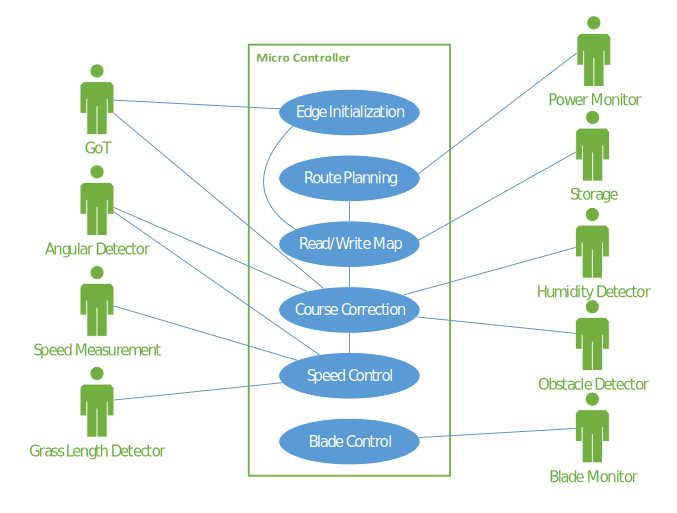
\includegraphics[scale=0.9]{figures/P5UseCase.pdf}
	\caption{Use-Case Diagram}
	\label{fig:usecase}
	\flushleft
\end{figure}

\noindent
The main purpose of the system is to automatically navigate in a specific area. In which area to navigate is set up by the \textit{edge initialization} functionality. This functionality handles the marking of the areas edges. This functionality only has to be used in the initialization process of the system. The concept is to only use the functionality after the GoT system has been positioned in the area. The consumer then takes the system around the edges of the area, while the GoT system tracks its positions. It is therefore only necessary to used this functionality, and for the consumer to walk with the system around the areas edges, if the GoT system has been moved. While the edge is being tracked, the \textit{edge initialization} uses the \textit{store map} functionality to store the information collected, in storage. \\\\ 
\noindent
The route to navigate after, in the specific area, is provided by the functionality \textit{route planning}. \textit{Route planning} uses the information, about the specific area, which is collected from the storage, to plan the most optimal route in which to follow. Furthermore the \textit{route planning} needs information about the systems power level to insure the functionality is considering if the system needs charging and therefore have to return to the charging station at some point on the route.\\\\
\noindent
The \textit{store map} functionality as described earlier, handles the communication with storage. Hence it stores information, received from the \textit{edge initialization} and collects information from storage when the functionality \textit{route planning} needs it. \\\\
\noindent
To insure the system is moving with a desired speed (in a straight line and in a turn) or a speed which is fitted to the height of the grass, detected with the \textit{grass length detector}, a \textit{speed control} functionality is necessary in the system. To insure the \textit{speed control} can deliver the desired speed an \textit{angular sensor} is utilized. \\\\
\noindent
The last functionality, \textit{course correction} is used when the system strays of the path calculated by \textit{route planning} or if the path gets blocked.
The obstacle which is blocking the route is detected by the sensor \textit{obstacle detector}. Furthermore the GoT system and the \textit{angular detector} will detect if the system is not on the desired path, or if the system starts to slip. Also, if it starts to rain, which is detected by the \textit{rain detector}, the system has to return to the charging station.
The \textit{course correction} sends the calculated data to the functionality \textit{speed control}. Hence the \textit{course correction} is the brain and the \textit{speed control} is the muscles.\\\\

\section{Prototype Constraints}
Before the prototype can be established, some considerations has to be made in respect to the time limitations and the main scope of this semester. The aim of the project is to create a functional proof of concept prototype of an automated lawn mower. The following section includes a brief description of the technology on which the prototype is constructed, along with argumentation for eliminated functionalities.

\subsection{Technology Base}
The technology which has been provided for the prototype is a tracked vehicle, seen on \figref{TrackedVehicle}. The vehicle comes with a brushed DC motor which provides power for rotation of the wheels, connected with the belts, and a servo motor which utilize breaks, connected to the wheels, to control the ratio of the differential steering. Furthermore the tracked vehicle includes two hall sensors, one by each belt, which keeps track of the speed, of the belts, by measuring pulses from magnets mounted on the front wheels. The testing will take place in Aalborg University Vicon Room, where the GoT system is installed and calibrated with the appurtenant transmitter, which is mounted on the tracked vehicle during test.

\begin{figure}[H]
	\centering
	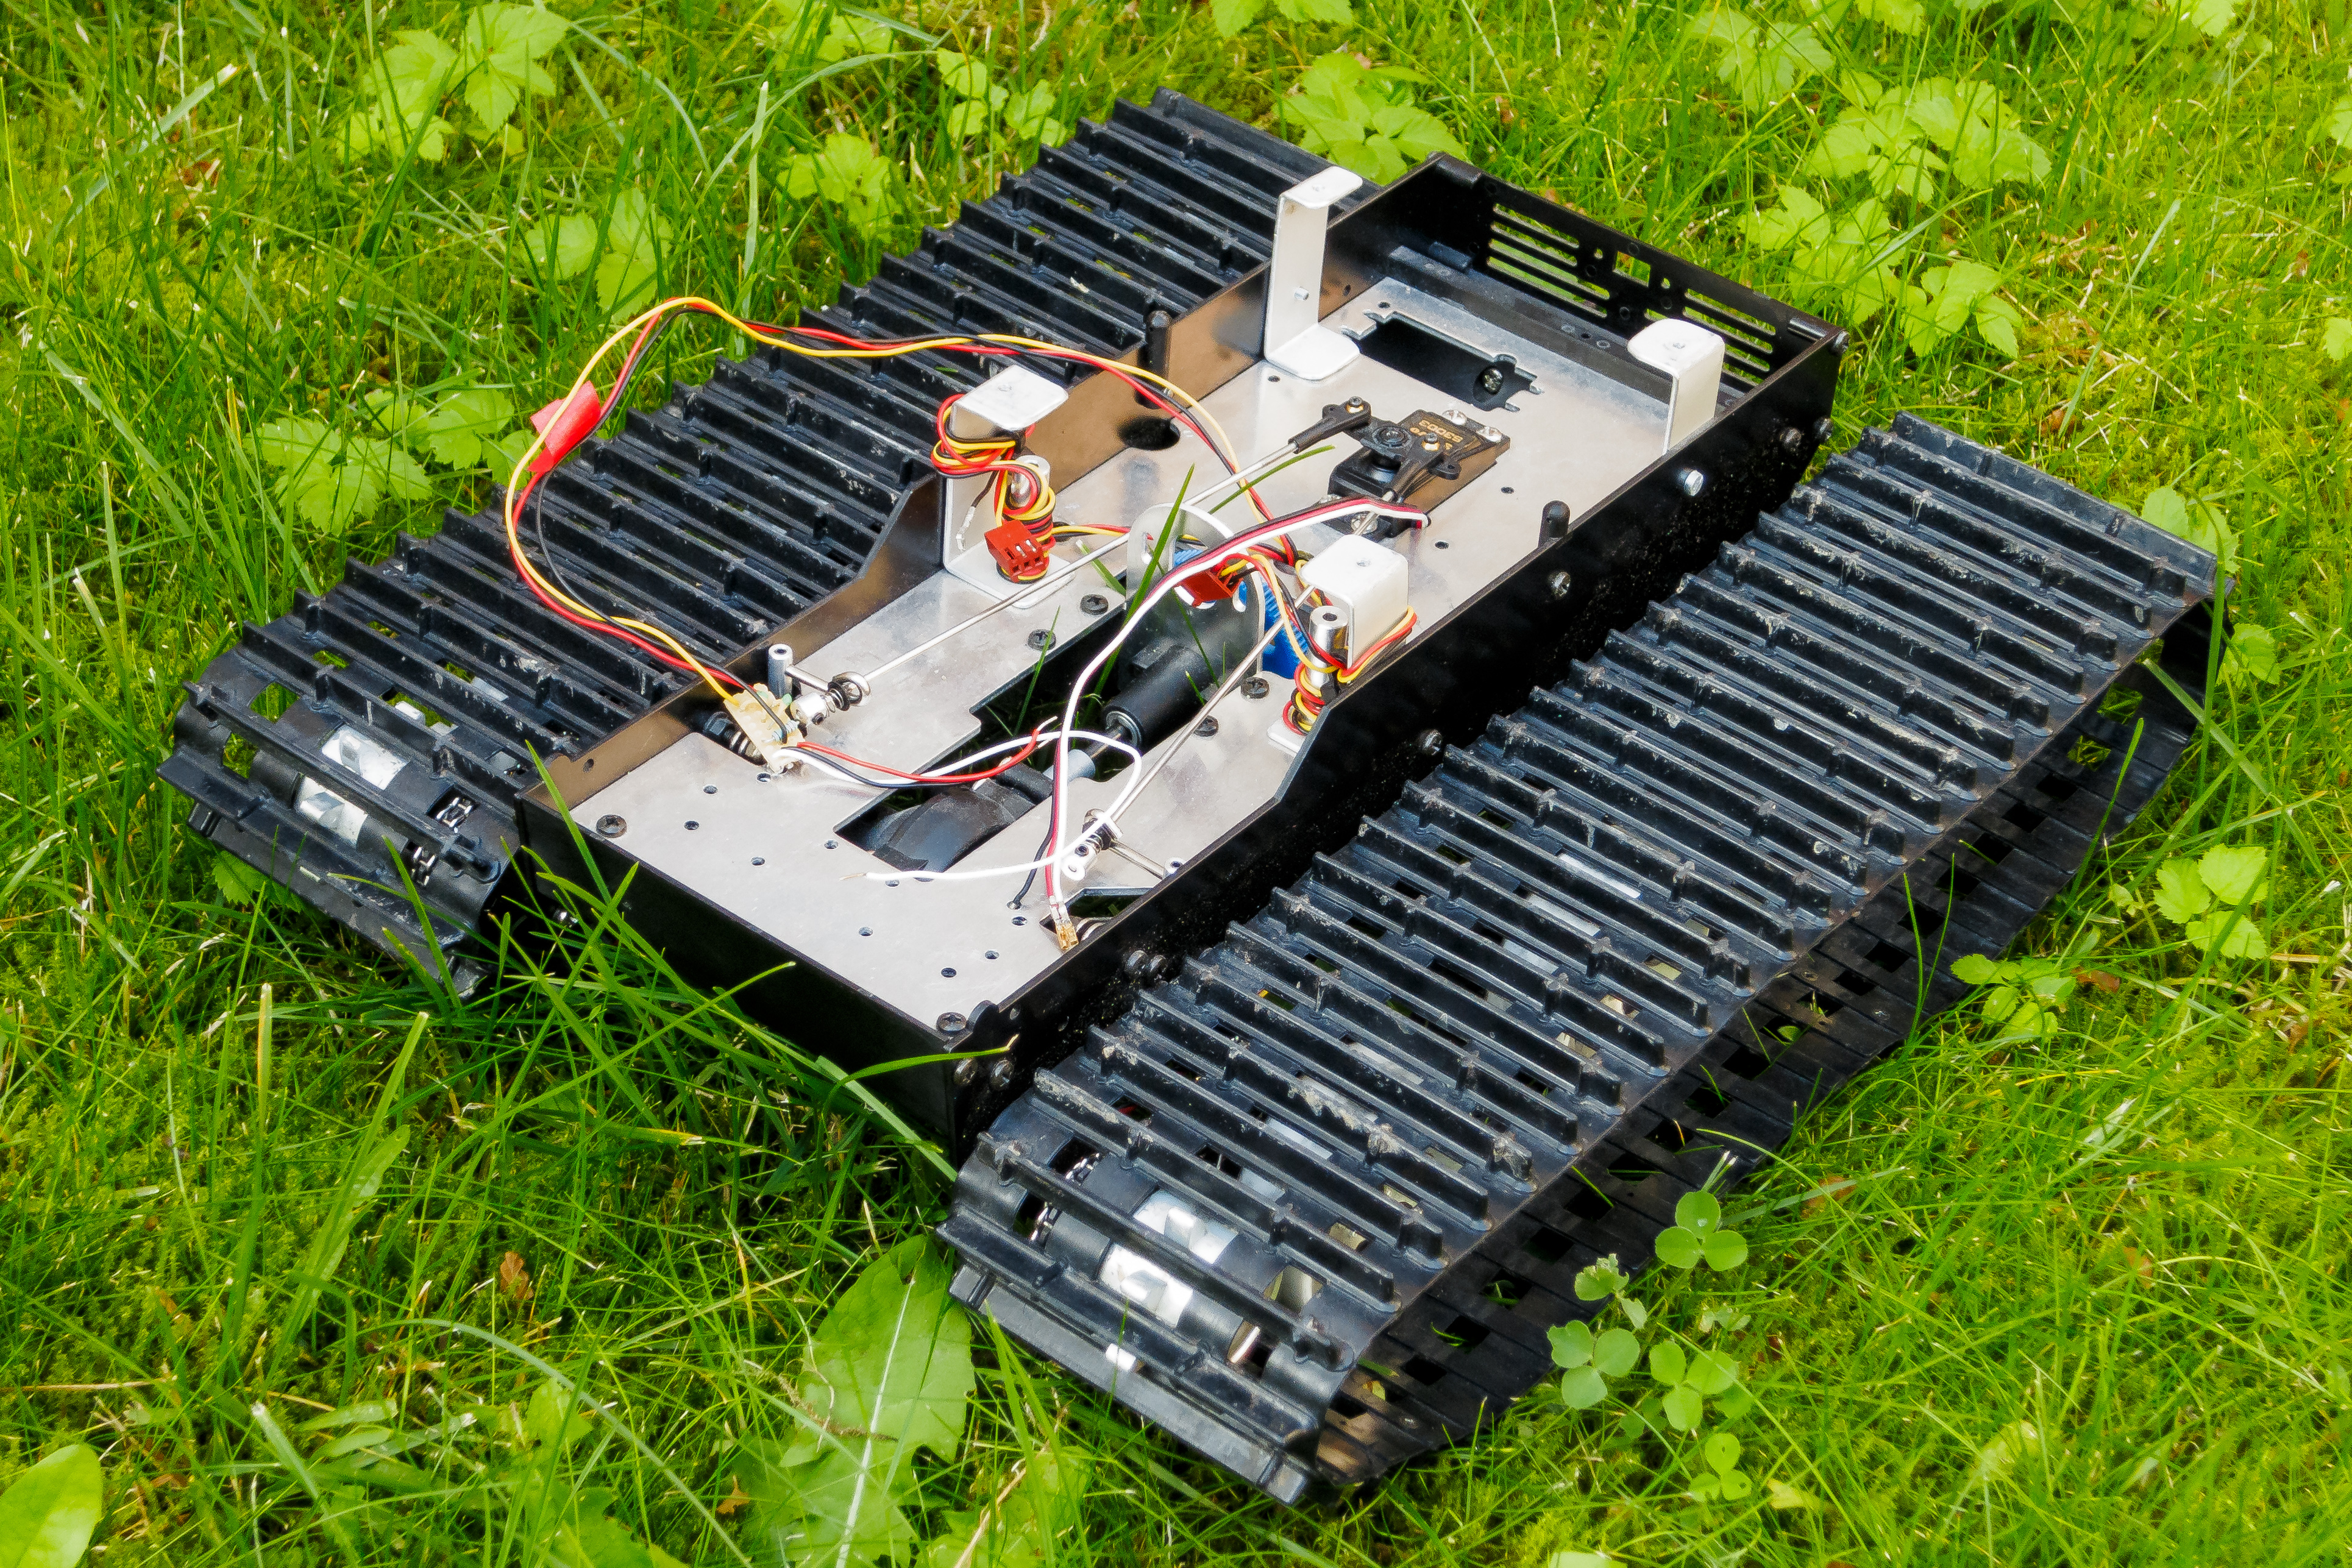
\includegraphics[scale=0.1]{figures/BeltVehicle.jpg}
	\flushleft
	\caption{Tracked vehicle with a brushed DC - and servomotor\fxnote{Insert picture of technology base}}
	\label{TrackedVehicle}
\end{figure}

\subsection{Grass Length Detection}
Detection of the grass length to control the speed of the lawn mower thus ensuring an evenly cut lawn, is a submodule which can be added at any time. Since it is not fatal for a working system and might even be unnecessary depending on time between each mowing of the lawn, it is decided to exclude this functionality from the initial design.

\subsection{Rain Sensor}
As the lawn mower is supposed to work outside, it is important to consider that it may be raining, and that an electronic device can be affected by those environmental issues. Even if the electrical part is waterproofed, there is a mechanical threat, a rain sensor could then warn the system to order the vehicle to get back in time.
It is possible to build the vehicle aware of those issues and add mechanical modules to secure it. However, the prototype will only be tested indoor, so this type of sensor will not be necessary in a prototype design.

\subsection{Obstacle Avoidance}
The lawn movers path might not always be clear, there could be some garden tools, tables or chairs, or people walking in it. The vehicle should be aware of what is in front of it at any time, to correct its path and get around the obstacle if necessary. To avoid this the sensor could be a pushing button to detect a solid strong object, or an ultrasound detector if the object is breakable.
As the aim of the project is to control the path of the vehicle by using angular positioning sensors, a proximity sensor will not be included. Static objects could be registered on the map to avoid these issues.\\\\
Furthermore the edge mapping functionality will not be included in the project which instead will focus on a quadratic map predefined in the test room.

\subsection{Power Monitoring}
Power monitoring could be implemented by measuring the voltage across the batteries, to ensure that the lawn mower is not running out of power, and to ensure the vehicles calculated route passes the charging station before the power runs too low.
This and the charging station will not be in the prototype, since it is beyond the scope of the project this semester and is not crucial for a working prototype.

\subsection{Prototype}
The overall functionalities for the project has been limited, due to time limitations and a desire to focus in the scope of the project. In this project a prototype will therefore be made to show the main functionalities necessary to make a automated vehicle.

The final prototype is to contain a regulator which will make it possible to follow a path from A to B. It will be able to continue if the transmission is lost between the prototype and the GoT system for a while. Furthermore it should be able to store data points from the GoT system.

%%it used as an indoor prototype, and in worse case, the last position of the vehicle 
%%will be recorded. The user can then take it by hand and plug it into the charging
%%station.
\input{contents/chapter2/Prototype.tex}


%---------- Chapter 3 ----------------------------------------
\chapter{Introduction}
\section{Household robots in general}
More and more robots appear in everyday life. Automatic vacuum cleaners and floor washers are getting widespread, as the technology is becoming cheaper and better. The vacuum cleaners have matured to a level, where they are been considered for saving man-hours in the elderly care sector.\\

\noindent
Outside the walls of our homes lays the next weekly hurdle: Mowing the lawn. A known way to handle this, is to pay the neighbour's teenager to do it. Unfortunately they grow up and move out, leaving the lawns in the residential neighbourhoods behind.\\ 

\noindent
Luckily engineers has stepped in, and provided a more long-term solution: Robotic lawn mowers.

\section{Robotic lawn mowers}
Several manufacturers of electrical gardening machines have started selling robotic lawn mowers in the recent years. In general they use one of two strategies when cutting the lawn:
\begin{itemize}
	\item Random direction mowers
	\item Parallel line mowers
\end{itemize}

\noindent
Mowers using the random direction strategy will drive in a straight line until a guard wire or an obstacle is detected. They will then turn in a random direction, and continue. See \figref{fig:randomcut}

\begin{figure}[H]
\centering
\includegraphics[scale=0.8]{figures/noLogicut.jpg} 
\label{fig:randomcut}
\caption{Random cut system [source:Bosch]} 
\end{figure}

\noindent
When the battery is nearly discharged, the mower will follow the guard wire back to the base station for recharging.\\

\noindent
Parallel line mowers uses a more intelligent control algorithm to optimize the mowing. After an initial learning run, following the guard wire around the lawn to be mowed, it will map the lawn, and cut in parallel lines, see \figref{fig:logicut}. The advantage of this strategy efficiency, as the lawn mower will not run over the same spots more than once. According to Bosch, a given lawn can be mowed up to 30\% faster with their Logicut system.
%% TODO: Insert source
 

\begin{figure}[H]
\centering
\includegraphics[scale=0.8]{figures/logicut.jpg} 
\label{fig:logicut}
\caption{Bosch Logicut system [source:Bosch]} 
\end{figure}

\noindent
Common for both systems is the guard wire, which has to be placed around the lawn and anywhere the lawn mower is not allowed to go, like flower beds, swimming pools, etc. \\

\noindent
This brings us to the problem with existing products.

\section{Problems with existing robotic lawn mowers}
All commercially available robotic lawn mowers requires a guard wire placed around the lawn. This can either be placed at the surface, and be held in place by pegs, or dug down below the surface. The guard wire must be routed around flower beds, etc. as well, see \figref{fig:robomow}

 
\begin{figure}[H]
\centering
\includegraphics[scale=0.6]{figures/robomow.png} 
\label{fig:robomow}
\caption{Guard wire installation [source:Robomow]} 
\end{figure}
\noindent

The use of the guard wire for guiding the mower back to the charging station presents another potential problem: In a garden with many restricted areas, the guard wire could get very long. This could therefore make the journey home long, compared to a more direct route. This again uses more battery power, that instead could have been used for actually mowing the lawn.\\

\noindent
This will be the motivation for the project: To avoid the work routing a wire around the garden, and as a bonus get more work done on a battery charge, by not wasting power following the wire home. 
    
\section{The Games on Track (GoT) system}
We were provided with the 'Games on Track GT-Position' system as a start to be able to figure out the lawn mower position in space.\\\\
It is composed of four different parts both hardware and software :
\begin{itemize}
	\item The tracked module, which emits ultra-sound waves. It should be placed on our lawn mower itself, so that the emitting cell is not obstructed by anything.
	\item Some beacons or receivers, placed all around the place the lawn mower will move in. Depending on the terrain, we can use from 2 to more than 20 of these : the more we place, the more accuracy we can get to fight against any ambient noise.
	\item The central system which gathers information about the distance of the tracked module to each beacon and transmits it to the computer via USB in regular intervals.
	\item The GoT software aggregates the received positions thoughout time and can be used to draw a map of the terrain (the lawn) and send every needed information to a third-party (our) piece of software.
\end{itemize}
GoT was firstly designed for train modeling but it is easily adaptable for any use of position tracking and seems a good choice, at first, for our autonomous lawn mower.

\section{Why not satellite positioning system ?}
The reasons why satellite positioning system won't be used in our project are mainly related to accuracy and energy consumption.\\\\
Indeed, these kinds of system like GPS or GLONASS would require a dedicated chip to put on the final system. The problem then would be the lack of precision under a few meters (around 2 or 3 meters in ideal situations for the best chips). \\\\
% TODO : Add reference to "A Review of GLONASS" Miller, 2000 & http://www.gps.gov/systems/gps/performance/accuracy/ %
Moreover, this kind of system implies slow communications with different distant satellites at the same time. Therefore, the energy consumption would quickly rise, thus reducing the lawn mower autonomy, which is not desirable.

\section{Potential consumer expectations}
The design of a product has no real value if no one is interested in using it. Thus, choices made during this project have to be made in accordance with the final user's expectations.\\\\
For instance, we need to keep in mind considerations regarding the autonomy of the vehicle (both in energy and for the navigation), but also towards the overall cost (\emph{insert price approximation here}). Even though, the GoT system itself has a cost beyond anything a normal customer would pay for a lawn mower, it appears, at first, as a good solution for us in terms of accuracy and energy consumption compared to GPS-like systems which are also quite expensive (\emph{insert price approximation here}). \\\\
For an improvement, we could consider replacing it with a similar solution as it is only a simple brick of the whole system. \emph{(This sentence should be perhaps moved to a dedicated part of the report)}\\\\
These are the types of preliminary considerations that will influence our design process for an autonomous lawn mower.

%---------- Chapter 4 ----------------------------------------
\chapter{Introduction}
\section{Household robots in general}
More and more robots appear in everyday life. Automatic vacuum cleaners and floor washers are getting widespread, as the technology is becoming cheaper and better. The vacuum cleaners have matured to a level, where they are been considered for saving man-hours in the elderly care sector.\\

\noindent
Outside the walls of our homes lays the next weekly hurdle: Mowing the lawn. A known way to handle this, is to pay the neighbour's teenager to do it. Unfortunately they grow up and move out, leaving the lawns in the residential neighbourhoods behind.\\ 

\noindent
Luckily engineers has stepped in, and provided a more long-term solution: Robotic lawn mowers.

\section{Robotic lawn mowers}
Several manufacturers of electrical gardening machines have started selling robotic lawn mowers in the recent years. In general they use one of two strategies when cutting the lawn:
\begin{itemize}
	\item Random direction mowers
	\item Parallel line mowers
\end{itemize}

\noindent
Mowers using the random direction strategy will drive in a straight line until a guard wire or an obstacle is detected. They will then turn in a random direction, and continue. See \figref{fig:randomcut}

\begin{figure}[H]
\centering
\includegraphics[scale=0.8]{figures/noLogicut.jpg} 
\label{fig:randomcut}
\caption{Random cut system [source:Bosch]} 
\end{figure}

\noindent
When the battery is nearly discharged, the mower will follow the guard wire back to the base station for recharging.\\

\noindent
Parallel line mowers uses a more intelligent control algorithm to optimize the mowing. After an initial learning run, following the guard wire around the lawn to be mowed, it will map the lawn, and cut in parallel lines, see \figref{fig:logicut}. The advantage of this strategy efficiency, as the lawn mower will not run over the same spots more than once. According to Bosch, a given lawn can be mowed up to 30\% faster with their Logicut system.
%% TODO: Insert source
 

\begin{figure}[H]
\centering
\includegraphics[scale=0.8]{figures/logicut.jpg} 
\label{fig:logicut}
\caption{Bosch Logicut system [source:Bosch]} 
\end{figure}

\noindent
Common for both systems is the guard wire, which has to be placed around the lawn and anywhere the lawn mower is not allowed to go, like flower beds, swimming pools, etc. \\

\noindent
This brings us to the problem with existing products.

\section{Problems with existing robotic lawn mowers}
All commercially available robotic lawn mowers requires a guard wire placed around the lawn. This can either be placed at the surface, and be held in place by pegs, or dug down below the surface. The guard wire must be routed around flower beds, etc. as well, see \figref{fig:robomow}

 
\begin{figure}[H]
\centering
\includegraphics[scale=0.6]{figures/robomow.png} 
\label{fig:robomow}
\caption{Guard wire installation [source:Robomow]} 
\end{figure}
\noindent

The use of the guard wire for guiding the mower back to the charging station presents another potential problem: In a garden with many restricted areas, the guard wire could get very long. This could therefore make the journey home long, compared to a more direct route. This again uses more battery power, that instead could have been used for actually mowing the lawn.\\

\noindent
This will be the motivation for the project: To avoid the work routing a wire around the garden, and as a bonus get more work done on a battery charge, by not wasting power following the wire home. 
    
\section{The Games on Track (GoT) system}
We were provided with the 'Games on Track GT-Position' system as a start to be able to figure out the lawn mower position in space.\\\\
It is composed of four different parts both hardware and software :
\begin{itemize}
	\item The tracked module, which emits ultra-sound waves. It should be placed on our lawn mower itself, so that the emitting cell is not obstructed by anything.
	\item Some beacons or receivers, placed all around the place the lawn mower will move in. Depending on the terrain, we can use from 2 to more than 20 of these : the more we place, the more accuracy we can get to fight against any ambient noise.
	\item The central system which gathers information about the distance of the tracked module to each beacon and transmits it to the computer via USB in regular intervals.
	\item The GoT software aggregates the received positions thoughout time and can be used to draw a map of the terrain (the lawn) and send every needed information to a third-party (our) piece of software.
\end{itemize}
GoT was firstly designed for train modeling but it is easily adaptable for any use of position tracking and seems a good choice, at first, for our autonomous lawn mower.

\section{Why not satellite positioning system ?}
The reasons why satellite positioning system won't be used in our project are mainly related to accuracy and energy consumption.\\\\
Indeed, these kinds of system like GPS or GLONASS would require a dedicated chip to put on the final system. The problem then would be the lack of precision under a few meters (around 2 or 3 meters in ideal situations for the best chips). \\\\
% TODO : Add reference to "A Review of GLONASS" Miller, 2000 & http://www.gps.gov/systems/gps/performance/accuracy/ %
Moreover, this kind of system implies slow communications with different distant satellites at the same time. Therefore, the energy consumption would quickly rise, thus reducing the lawn mower autonomy, which is not desirable.

\section{Potential consumer expectations}
The design of a product has no real value if no one is interested in using it. Thus, choices made during this project have to be made in accordance with the final user's expectations.\\\\
For instance, we need to keep in mind considerations regarding the autonomy of the vehicle (both in energy and for the navigation), but also towards the overall cost (\emph{insert price approximation here}). Even though, the GoT system itself has a cost beyond anything a normal customer would pay for a lawn mower, it appears, at first, as a good solution for us in terms of accuracy and energy consumption compared to GPS-like systems which are also quite expensive (\emph{insert price approximation here}). \\\\
For an improvement, we could consider replacing it with a similar solution as it is only a simple brick of the whole system. \emph{(This sentence should be perhaps moved to a dedicated part of the report)}\\\\
These are the types of preliminary considerations that will influence our design process for an autonomous lawn mower.

%---------- Chapter 5 ----------------------------------------
\chapter{Introduction}
\section{Household robots in general}
More and more robots appear in everyday life. Automatic vacuum cleaners and floor washers are getting widespread, as the technology is becoming cheaper and better. The vacuum cleaners have matured to a level, where they are been considered for saving man-hours in the elderly care sector.\\

\noindent
Outside the walls of our homes lays the next weekly hurdle: Mowing the lawn. A known way to handle this, is to pay the neighbour's teenager to do it. Unfortunately they grow up and move out, leaving the lawns in the residential neighbourhoods behind.\\ 

\noindent
Luckily engineers has stepped in, and provided a more long-term solution: Robotic lawn mowers.

\section{Robotic lawn mowers}
Several manufacturers of electrical gardening machines have started selling robotic lawn mowers in the recent years. In general they use one of two strategies when cutting the lawn:
\begin{itemize}
	\item Random direction mowers
	\item Parallel line mowers
\end{itemize}

\noindent
Mowers using the random direction strategy will drive in a straight line until a guard wire or an obstacle is detected. They will then turn in a random direction, and continue. See \figref{fig:randomcut}

\begin{figure}[H]
\centering
\includegraphics[scale=0.8]{figures/noLogicut.jpg} 
\label{fig:randomcut}
\caption{Random cut system [source:Bosch]} 
\end{figure}

\noindent
When the battery is nearly discharged, the mower will follow the guard wire back to the base station for recharging.\\

\noindent
Parallel line mowers uses a more intelligent control algorithm to optimize the mowing. After an initial learning run, following the guard wire around the lawn to be mowed, it will map the lawn, and cut in parallel lines, see \figref{fig:logicut}. The advantage of this strategy efficiency, as the lawn mower will not run over the same spots more than once. According to Bosch, a given lawn can be mowed up to 30\% faster with their Logicut system.
%% TODO: Insert source
 

\begin{figure}[H]
\centering
\includegraphics[scale=0.8]{figures/logicut.jpg} 
\label{fig:logicut}
\caption{Bosch Logicut system [source:Bosch]} 
\end{figure}

\noindent
Common for both systems is the guard wire, which has to be placed around the lawn and anywhere the lawn mower is not allowed to go, like flower beds, swimming pools, etc. \\

\noindent
This brings us to the problem with existing products.

\section{Problems with existing robotic lawn mowers}
All commercially available robotic lawn mowers requires a guard wire placed around the lawn. This can either be placed at the surface, and be held in place by pegs, or dug down below the surface. The guard wire must be routed around flower beds, etc. as well, see \figref{fig:robomow}

 
\begin{figure}[H]
\centering
\includegraphics[scale=0.6]{figures/robomow.png} 
\label{fig:robomow}
\caption{Guard wire installation [source:Robomow]} 
\end{figure}
\noindent

The use of the guard wire for guiding the mower back to the charging station presents another potential problem: In a garden with many restricted areas, the guard wire could get very long. This could therefore make the journey home long, compared to a more direct route. This again uses more battery power, that instead could have been used for actually mowing the lawn.\\

\noindent
This will be the motivation for the project: To avoid the work routing a wire around the garden, and as a bonus get more work done on a battery charge, by not wasting power following the wire home. 
    
\section{The Games on Track (GoT) system}
We were provided with the 'Games on Track GT-Position' system as a start to be able to figure out the lawn mower position in space.\\\\
It is composed of four different parts both hardware and software :
\begin{itemize}
	\item The tracked module, which emits ultra-sound waves. It should be placed on our lawn mower itself, so that the emitting cell is not obstructed by anything.
	\item Some beacons or receivers, placed all around the place the lawn mower will move in. Depending on the terrain, we can use from 2 to more than 20 of these : the more we place, the more accuracy we can get to fight against any ambient noise.
	\item The central system which gathers information about the distance of the tracked module to each beacon and transmits it to the computer via USB in regular intervals.
	\item The GoT software aggregates the received positions thoughout time and can be used to draw a map of the terrain (the lawn) and send every needed information to a third-party (our) piece of software.
\end{itemize}
GoT was firstly designed for train modeling but it is easily adaptable for any use of position tracking and seems a good choice, at first, for our autonomous lawn mower.

\section{Why not satellite positioning system ?}
The reasons why satellite positioning system won't be used in our project are mainly related to accuracy and energy consumption.\\\\
Indeed, these kinds of system like GPS or GLONASS would require a dedicated chip to put on the final system. The problem then would be the lack of precision under a few meters (around 2 or 3 meters in ideal situations for the best chips). \\\\
% TODO : Add reference to "A Review of GLONASS" Miller, 2000 & http://www.gps.gov/systems/gps/performance/accuracy/ %
Moreover, this kind of system implies slow communications with different distant satellites at the same time. Therefore, the energy consumption would quickly rise, thus reducing the lawn mower autonomy, which is not desirable.

\section{Potential consumer expectations}
The design of a product has no real value if no one is interested in using it. Thus, choices made during this project have to be made in accordance with the final user's expectations.\\\\
For instance, we need to keep in mind considerations regarding the autonomy of the vehicle (both in energy and for the navigation), but also towards the overall cost (\emph{insert price approximation here}). Even though, the GoT system itself has a cost beyond anything a normal customer would pay for a lawn mower, it appears, at first, as a good solution for us in terms of accuracy and energy consumption compared to GPS-like systems which are also quite expensive (\emph{insert price approximation here}). \\\\
For an improvement, we could consider replacing it with a similar solution as it is only a simple brick of the whole system. \emph{(This sentence should be perhaps moved to a dedicated part of the report)}\\\\
These are the types of preliminary considerations that will influence our design process for an autonomous lawn mower.

%---------- Chapter 6 ----------------------------------------
\chapter{Introduction}
\section{Household robots in general}
More and more robots appear in everyday life. Automatic vacuum cleaners and floor washers are getting widespread, as the technology is becoming cheaper and better. The vacuum cleaners have matured to a level, where they are been considered for saving man-hours in the elderly care sector.\\

\noindent
Outside the walls of our homes lays the next weekly hurdle: Mowing the lawn. A known way to handle this, is to pay the neighbour's teenager to do it. Unfortunately they grow up and move out, leaving the lawns in the residential neighbourhoods behind.\\ 

\noindent
Luckily engineers has stepped in, and provided a more long-term solution: Robotic lawn mowers.

\section{Robotic lawn mowers}
Several manufacturers of electrical gardening machines have started selling robotic lawn mowers in the recent years. In general they use one of two strategies when cutting the lawn:
\begin{itemize}
	\item Random direction mowers
	\item Parallel line mowers
\end{itemize}

\noindent
Mowers using the random direction strategy will drive in a straight line until a guard wire or an obstacle is detected. They will then turn in a random direction, and continue. See \figref{fig:randomcut}

\begin{figure}[H]
\centering
\includegraphics[scale=0.8]{figures/noLogicut.jpg} 
\label{fig:randomcut}
\caption{Random cut system [source:Bosch]} 
\end{figure}

\noindent
When the battery is nearly discharged, the mower will follow the guard wire back to the base station for recharging.\\

\noindent
Parallel line mowers uses a more intelligent control algorithm to optimize the mowing. After an initial learning run, following the guard wire around the lawn to be mowed, it will map the lawn, and cut in parallel lines, see \figref{fig:logicut}. The advantage of this strategy efficiency, as the lawn mower will not run over the same spots more than once. According to Bosch, a given lawn can be mowed up to 30\% faster with their Logicut system.
%% TODO: Insert source
 

\begin{figure}[H]
\centering
\includegraphics[scale=0.8]{figures/logicut.jpg} 
\label{fig:logicut}
\caption{Bosch Logicut system [source:Bosch]} 
\end{figure}

\noindent
Common for both systems is the guard wire, which has to be placed around the lawn and anywhere the lawn mower is not allowed to go, like flower beds, swimming pools, etc. \\

\noindent
This brings us to the problem with existing products.

\section{Problems with existing robotic lawn mowers}
All commercially available robotic lawn mowers requires a guard wire placed around the lawn. This can either be placed at the surface, and be held in place by pegs, or dug down below the surface. The guard wire must be routed around flower beds, etc. as well, see \figref{fig:robomow}

 
\begin{figure}[H]
\centering
\includegraphics[scale=0.6]{figures/robomow.png} 
\label{fig:robomow}
\caption{Guard wire installation [source:Robomow]} 
\end{figure}
\noindent

The use of the guard wire for guiding the mower back to the charging station presents another potential problem: In a garden with many restricted areas, the guard wire could get very long. This could therefore make the journey home long, compared to a more direct route. This again uses more battery power, that instead could have been used for actually mowing the lawn.\\

\noindent
This will be the motivation for the project: To avoid the work routing a wire around the garden, and as a bonus get more work done on a battery charge, by not wasting power following the wire home. 
    
\section{The Games on Track (GoT) system}
We were provided with the 'Games on Track GT-Position' system as a start to be able to figure out the lawn mower position in space.\\\\
It is composed of four different parts both hardware and software :
\begin{itemize}
	\item The tracked module, which emits ultra-sound waves. It should be placed on our lawn mower itself, so that the emitting cell is not obstructed by anything.
	\item Some beacons or receivers, placed all around the place the lawn mower will move in. Depending on the terrain, we can use from 2 to more than 20 of these : the more we place, the more accuracy we can get to fight against any ambient noise.
	\item The central system which gathers information about the distance of the tracked module to each beacon and transmits it to the computer via USB in regular intervals.
	\item The GoT software aggregates the received positions thoughout time and can be used to draw a map of the terrain (the lawn) and send every needed information to a third-party (our) piece of software.
\end{itemize}
GoT was firstly designed for train modeling but it is easily adaptable for any use of position tracking and seems a good choice, at first, for our autonomous lawn mower.

\section{Why not satellite positioning system ?}
The reasons why satellite positioning system won't be used in our project are mainly related to accuracy and energy consumption.\\\\
Indeed, these kinds of system like GPS or GLONASS would require a dedicated chip to put on the final system. The problem then would be the lack of precision under a few meters (around 2 or 3 meters in ideal situations for the best chips). \\\\
% TODO : Add reference to "A Review of GLONASS" Miller, 2000 & http://www.gps.gov/systems/gps/performance/accuracy/ %
Moreover, this kind of system implies slow communications with different distant satellites at the same time. Therefore, the energy consumption would quickly rise, thus reducing the lawn mower autonomy, which is not desirable.

\section{Potential consumer expectations}
The design of a product has no real value if no one is interested in using it. Thus, choices made during this project have to be made in accordance with the final user's expectations.\\\\
For instance, we need to keep in mind considerations regarding the autonomy of the vehicle (both in energy and for the navigation), but also towards the overall cost (\emph{insert price approximation here}). Even though, the GoT system itself has a cost beyond anything a normal customer would pay for a lawn mower, it appears, at first, as a good solution for us in terms of accuracy and energy consumption compared to GPS-like systems which are also quite expensive (\emph{insert price approximation here}). \\\\
For an improvement, we could consider replacing it with a similar solution as it is only a simple brick of the whole system. \emph{(This sentence should be perhaps moved to a dedicated part of the report)}\\\\
These are the types of preliminary considerations that will influence our design process for an autonomous lawn mower.

%---------- Chapter 7 ----------------------------------------
\chapter{Introduction}
\section{Household robots in general}
More and more robots appear in everyday life. Automatic vacuum cleaners and floor washers are getting widespread, as the technology is becoming cheaper and better. The vacuum cleaners have matured to a level, where they are been considered for saving man-hours in the elderly care sector.\\

\noindent
Outside the walls of our homes lays the next weekly hurdle: Mowing the lawn. A known way to handle this, is to pay the neighbour's teenager to do it. Unfortunately they grow up and move out, leaving the lawns in the residential neighbourhoods behind.\\ 

\noindent
Luckily engineers has stepped in, and provided a more long-term solution: Robotic lawn mowers.

\section{Robotic lawn mowers}
Several manufacturers of electrical gardening machines have started selling robotic lawn mowers in the recent years. In general they use one of two strategies when cutting the lawn:
\begin{itemize}
	\item Random direction mowers
	\item Parallel line mowers
\end{itemize}

\noindent
Mowers using the random direction strategy will drive in a straight line until a guard wire or an obstacle is detected. They will then turn in a random direction, and continue. See \figref{fig:randomcut}

\begin{figure}[H]
\centering
\includegraphics[scale=0.8]{figures/noLogicut.jpg} 
\label{fig:randomcut}
\caption{Random cut system [source:Bosch]} 
\end{figure}

\noindent
When the battery is nearly discharged, the mower will follow the guard wire back to the base station for recharging.\\

\noindent
Parallel line mowers uses a more intelligent control algorithm to optimize the mowing. After an initial learning run, following the guard wire around the lawn to be mowed, it will map the lawn, and cut in parallel lines, see \figref{fig:logicut}. The advantage of this strategy efficiency, as the lawn mower will not run over the same spots more than once. According to Bosch, a given lawn can be mowed up to 30\% faster with their Logicut system.
%% TODO: Insert source
 

\begin{figure}[H]
\centering
\includegraphics[scale=0.8]{figures/logicut.jpg} 
\label{fig:logicut}
\caption{Bosch Logicut system [source:Bosch]} 
\end{figure}

\noindent
Common for both systems is the guard wire, which has to be placed around the lawn and anywhere the lawn mower is not allowed to go, like flower beds, swimming pools, etc. \\

\noindent
This brings us to the problem with existing products.

\section{Problems with existing robotic lawn mowers}
All commercially available robotic lawn mowers requires a guard wire placed around the lawn. This can either be placed at the surface, and be held in place by pegs, or dug down below the surface. The guard wire must be routed around flower beds, etc. as well, see \figref{fig:robomow}

 
\begin{figure}[H]
\centering
\includegraphics[scale=0.6]{figures/robomow.png} 
\label{fig:robomow}
\caption{Guard wire installation [source:Robomow]} 
\end{figure}
\noindent

The use of the guard wire for guiding the mower back to the charging station presents another potential problem: In a garden with many restricted areas, the guard wire could get very long. This could therefore make the journey home long, compared to a more direct route. This again uses more battery power, that instead could have been used for actually mowing the lawn.\\

\noindent
This will be the motivation for the project: To avoid the work routing a wire around the garden, and as a bonus get more work done on a battery charge, by not wasting power following the wire home. 
    
\section{The Games on Track (GoT) system}
We were provided with the 'Games on Track GT-Position' system as a start to be able to figure out the lawn mower position in space.\\\\
It is composed of four different parts both hardware and software :
\begin{itemize}
	\item The tracked module, which emits ultra-sound waves. It should be placed on our lawn mower itself, so that the emitting cell is not obstructed by anything.
	\item Some beacons or receivers, placed all around the place the lawn mower will move in. Depending on the terrain, we can use from 2 to more than 20 of these : the more we place, the more accuracy we can get to fight against any ambient noise.
	\item The central system which gathers information about the distance of the tracked module to each beacon and transmits it to the computer via USB in regular intervals.
	\item The GoT software aggregates the received positions thoughout time and can be used to draw a map of the terrain (the lawn) and send every needed information to a third-party (our) piece of software.
\end{itemize}
GoT was firstly designed for train modeling but it is easily adaptable for any use of position tracking and seems a good choice, at first, for our autonomous lawn mower.

\section{Why not satellite positioning system ?}
The reasons why satellite positioning system won't be used in our project are mainly related to accuracy and energy consumption.\\\\
Indeed, these kinds of system like GPS or GLONASS would require a dedicated chip to put on the final system. The problem then would be the lack of precision under a few meters (around 2 or 3 meters in ideal situations for the best chips). \\\\
% TODO : Add reference to "A Review of GLONASS" Miller, 2000 & http://www.gps.gov/systems/gps/performance/accuracy/ %
Moreover, this kind of system implies slow communications with different distant satellites at the same time. Therefore, the energy consumption would quickly rise, thus reducing the lawn mower autonomy, which is not desirable.

\section{Potential consumer expectations}
The design of a product has no real value if no one is interested in using it. Thus, choices made during this project have to be made in accordance with the final user's expectations.\\\\
For instance, we need to keep in mind considerations regarding the autonomy of the vehicle (both in energy and for the navigation), but also towards the overall cost (\emph{insert price approximation here}). Even though, the GoT system itself has a cost beyond anything a normal customer would pay for a lawn mower, it appears, at first, as a good solution for us in terms of accuracy and energy consumption compared to GPS-like systems which are also quite expensive (\emph{insert price approximation here}). \\\\
For an improvement, we could consider replacing it with a similar solution as it is only a simple brick of the whole system. \emph{(This sentence should be perhaps moved to a dedicated part of the report)}\\\\
These are the types of preliminary considerations that will influence our design process for an autonomous lawn mower.

%---------- Chapter 8 ----------------------------------------
\chapter{Introduction}
\section{Household robots in general}
More and more robots appear in everyday life. Automatic vacuum cleaners and floor washers are getting widespread, as the technology is becoming cheaper and better. The vacuum cleaners have matured to a level, where they are been considered for saving man-hours in the elderly care sector.\\

\noindent
Outside the walls of our homes lays the next weekly hurdle: Mowing the lawn. A known way to handle this, is to pay the neighbour's teenager to do it. Unfortunately they grow up and move out, leaving the lawns in the residential neighbourhoods behind.\\ 

\noindent
Luckily engineers has stepped in, and provided a more long-term solution: Robotic lawn mowers.

\section{Robotic lawn mowers}
Several manufacturers of electrical gardening machines have started selling robotic lawn mowers in the recent years. In general they use one of two strategies when cutting the lawn:
\begin{itemize}
	\item Random direction mowers
	\item Parallel line mowers
\end{itemize}

\noindent
Mowers using the random direction strategy will drive in a straight line until a guard wire or an obstacle is detected. They will then turn in a random direction, and continue. See \figref{fig:randomcut}

\begin{figure}[H]
\centering
\includegraphics[scale=0.8]{figures/noLogicut.jpg} 
\label{fig:randomcut}
\caption{Random cut system [source:Bosch]} 
\end{figure}

\noindent
When the battery is nearly discharged, the mower will follow the guard wire back to the base station for recharging.\\

\noindent
Parallel line mowers uses a more intelligent control algorithm to optimize the mowing. After an initial learning run, following the guard wire around the lawn to be mowed, it will map the lawn, and cut in parallel lines, see \figref{fig:logicut}. The advantage of this strategy efficiency, as the lawn mower will not run over the same spots more than once. According to Bosch, a given lawn can be mowed up to 30\% faster with their Logicut system.
%% TODO: Insert source
 

\begin{figure}[H]
\centering
\includegraphics[scale=0.8]{figures/logicut.jpg} 
\label{fig:logicut}
\caption{Bosch Logicut system [source:Bosch]} 
\end{figure}

\noindent
Common for both systems is the guard wire, which has to be placed around the lawn and anywhere the lawn mower is not allowed to go, like flower beds, swimming pools, etc. \\

\noindent
This brings us to the problem with existing products.

\section{Problems with existing robotic lawn mowers}
All commercially available robotic lawn mowers requires a guard wire placed around the lawn. This can either be placed at the surface, and be held in place by pegs, or dug down below the surface. The guard wire must be routed around flower beds, etc. as well, see \figref{fig:robomow}

 
\begin{figure}[H]
\centering
\includegraphics[scale=0.6]{figures/robomow.png} 
\label{fig:robomow}
\caption{Guard wire installation [source:Robomow]} 
\end{figure}
\noindent

The use of the guard wire for guiding the mower back to the charging station presents another potential problem: In a garden with many restricted areas, the guard wire could get very long. This could therefore make the journey home long, compared to a more direct route. This again uses more battery power, that instead could have been used for actually mowing the lawn.\\

\noindent
This will be the motivation for the project: To avoid the work routing a wire around the garden, and as a bonus get more work done on a battery charge, by not wasting power following the wire home. 
    
\section{The Games on Track (GoT) system}
We were provided with the 'Games on Track GT-Position' system as a start to be able to figure out the lawn mower position in space.\\\\
It is composed of four different parts both hardware and software :
\begin{itemize}
	\item The tracked module, which emits ultra-sound waves. It should be placed on our lawn mower itself, so that the emitting cell is not obstructed by anything.
	\item Some beacons or receivers, placed all around the place the lawn mower will move in. Depending on the terrain, we can use from 2 to more than 20 of these : the more we place, the more accuracy we can get to fight against any ambient noise.
	\item The central system which gathers information about the distance of the tracked module to each beacon and transmits it to the computer via USB in regular intervals.
	\item The GoT software aggregates the received positions thoughout time and can be used to draw a map of the terrain (the lawn) and send every needed information to a third-party (our) piece of software.
\end{itemize}
GoT was firstly designed for train modeling but it is easily adaptable for any use of position tracking and seems a good choice, at first, for our autonomous lawn mower.

\section{Why not satellite positioning system ?}
The reasons why satellite positioning system won't be used in our project are mainly related to accuracy and energy consumption.\\\\
Indeed, these kinds of system like GPS or GLONASS would require a dedicated chip to put on the final system. The problem then would be the lack of precision under a few meters (around 2 or 3 meters in ideal situations for the best chips). \\\\
% TODO : Add reference to "A Review of GLONASS" Miller, 2000 & http://www.gps.gov/systems/gps/performance/accuracy/ %
Moreover, this kind of system implies slow communications with different distant satellites at the same time. Therefore, the energy consumption would quickly rise, thus reducing the lawn mower autonomy, which is not desirable.

\section{Potential consumer expectations}
The design of a product has no real value if no one is interested in using it. Thus, choices made during this project have to be made in accordance with the final user's expectations.\\\\
For instance, we need to keep in mind considerations regarding the autonomy of the vehicle (both in energy and for the navigation), but also towards the overall cost (\emph{insert price approximation here}). Even though, the GoT system itself has a cost beyond anything a normal customer would pay for a lawn mower, it appears, at first, as a good solution for us in terms of accuracy and energy consumption compared to GPS-like systems which are also quite expensive (\emph{insert price approximation here}). \\\\
For an improvement, we could consider replacing it with a similar solution as it is only a simple brick of the whole system. \emph{(This sentence should be perhaps moved to a dedicated part of the report)}\\\\
These are the types of preliminary considerations that will influence our design process for an autonomous lawn mower.

%---------- Chapter 9 ----------------------------------------
\chapter{Introduction}
\section{Household robots in general}
More and more robots appear in everyday life. Automatic vacuum cleaners and floor washers are getting widespread, as the technology is becoming cheaper and better. The vacuum cleaners have matured to a level, where they are been considered for saving man-hours in the elderly care sector.\\

\noindent
Outside the walls of our homes lays the next weekly hurdle: Mowing the lawn. A known way to handle this, is to pay the neighbour's teenager to do it. Unfortunately they grow up and move out, leaving the lawns in the residential neighbourhoods behind.\\ 

\noindent
Luckily engineers has stepped in, and provided a more long-term solution: Robotic lawn mowers.

\section{Robotic lawn mowers}
Several manufacturers of electrical gardening machines have started selling robotic lawn mowers in the recent years. In general they use one of two strategies when cutting the lawn:
\begin{itemize}
	\item Random direction mowers
	\item Parallel line mowers
\end{itemize}

\noindent
Mowers using the random direction strategy will drive in a straight line until a guard wire or an obstacle is detected. They will then turn in a random direction, and continue. See \figref{fig:randomcut}

\begin{figure}[H]
\centering
\includegraphics[scale=0.8]{figures/noLogicut.jpg} 
\label{fig:randomcut}
\caption{Random cut system [source:Bosch]} 
\end{figure}

\noindent
When the battery is nearly discharged, the mower will follow the guard wire back to the base station for recharging.\\

\noindent
Parallel line mowers uses a more intelligent control algorithm to optimize the mowing. After an initial learning run, following the guard wire around the lawn to be mowed, it will map the lawn, and cut in parallel lines, see \figref{fig:logicut}. The advantage of this strategy efficiency, as the lawn mower will not run over the same spots more than once. According to Bosch, a given lawn can be mowed up to 30\% faster with their Logicut system.
%% TODO: Insert source
 

\begin{figure}[H]
\centering
\includegraphics[scale=0.8]{figures/logicut.jpg} 
\label{fig:logicut}
\caption{Bosch Logicut system [source:Bosch]} 
\end{figure}

\noindent
Common for both systems is the guard wire, which has to be placed around the lawn and anywhere the lawn mower is not allowed to go, like flower beds, swimming pools, etc. \\

\noindent
This brings us to the problem with existing products.

\section{Problems with existing robotic lawn mowers}
All commercially available robotic lawn mowers requires a guard wire placed around the lawn. This can either be placed at the surface, and be held in place by pegs, or dug down below the surface. The guard wire must be routed around flower beds, etc. as well, see \figref{fig:robomow}

 
\begin{figure}[H]
\centering
\includegraphics[scale=0.6]{figures/robomow.png} 
\label{fig:robomow}
\caption{Guard wire installation [source:Robomow]} 
\end{figure}
\noindent

The use of the guard wire for guiding the mower back to the charging station presents another potential problem: In a garden with many restricted areas, the guard wire could get very long. This could therefore make the journey home long, compared to a more direct route. This again uses more battery power, that instead could have been used for actually mowing the lawn.\\

\noindent
This will be the motivation for the project: To avoid the work routing a wire around the garden, and as a bonus get more work done on a battery charge, by not wasting power following the wire home. 
    
\section{The Games on Track (GoT) system}
We were provided with the 'Games on Track GT-Position' system as a start to be able to figure out the lawn mower position in space.\\\\
It is composed of four different parts both hardware and software :
\begin{itemize}
	\item The tracked module, which emits ultra-sound waves. It should be placed on our lawn mower itself, so that the emitting cell is not obstructed by anything.
	\item Some beacons or receivers, placed all around the place the lawn mower will move in. Depending on the terrain, we can use from 2 to more than 20 of these : the more we place, the more accuracy we can get to fight against any ambient noise.
	\item The central system which gathers information about the distance of the tracked module to each beacon and transmits it to the computer via USB in regular intervals.
	\item The GoT software aggregates the received positions thoughout time and can be used to draw a map of the terrain (the lawn) and send every needed information to a third-party (our) piece of software.
\end{itemize}
GoT was firstly designed for train modeling but it is easily adaptable for any use of position tracking and seems a good choice, at first, for our autonomous lawn mower.

\section{Why not satellite positioning system ?}
The reasons why satellite positioning system won't be used in our project are mainly related to accuracy and energy consumption.\\\\
Indeed, these kinds of system like GPS or GLONASS would require a dedicated chip to put on the final system. The problem then would be the lack of precision under a few meters (around 2 or 3 meters in ideal situations for the best chips). \\\\
% TODO : Add reference to "A Review of GLONASS" Miller, 2000 & http://www.gps.gov/systems/gps/performance/accuracy/ %
Moreover, this kind of system implies slow communications with different distant satellites at the same time. Therefore, the energy consumption would quickly rise, thus reducing the lawn mower autonomy, which is not desirable.

\section{Potential consumer expectations}
The design of a product has no real value if no one is interested in using it. Thus, choices made during this project have to be made in accordance with the final user's expectations.\\\\
For instance, we need to keep in mind considerations regarding the autonomy of the vehicle (both in energy and for the navigation), but also towards the overall cost (\emph{insert price approximation here}). Even though, the GoT system itself has a cost beyond anything a normal customer would pay for a lawn mower, it appears, at first, as a good solution for us in terms of accuracy and energy consumption compared to GPS-like systems which are also quite expensive (\emph{insert price approximation here}). \\\\
For an improvement, we could consider replacing it with a similar solution as it is only a simple brick of the whole system. \emph{(This sentence should be perhaps moved to a dedicated part of the report)}\\\\
These are the types of preliminary considerations that will influence our design process for an autonomous lawn mower.


\cleardoublepage


%numbers the pages with appendix numeral - starts from "A.1":
\pagenumbering{Roman}

\cleardoublepage

%numbers the chapters with letters (A, B, C, etc.):
\appendix

%including appendix:
%---------- Appendix A ---------------------------------------
\input{appendix/aAppendix/aAppendix.tex}

%---------- Appendix B ---------------------------------------
\input{appendix/bAppendix/aAppendix.tex}

%---------- Appendix C ---------------------------------------
\input{appendix/cAppendix/aAppendix.tex}

%---------- Appendix D ---------------------------------------
\input{appendix/dAppendix/aAppendix.tex}

%---------- Appendix E ---------------------------------------
\input{appendix/eAppendix/aAppendix.tex}

%---------- Appendix F ---------------------------------------
\input{appendix/fAppendix/aAppendix.tex}

%---------- Appendix G ---------------------------------------
\input{appendix/gAppendix/aAppendix.tex}

%---------- Appendix H ---------------------------------------
\input{appendix/hAppendix/aAppendix.tex}

%bibliography is set to chicago-style (author, year of publication and page number is used for references):
%\renewcommand\finalnamedelim{\space og\space}
\printbibliography

\pagebreak

\section*{Glossary}
%\begin{itemize}
%  \item[-]
%\end{itemize}

\listoffixmes

\end{document}